\documentclass{article}

\usepackage{amsmath, amsthm, amssymb, amsfonts}
\usepackage{bm}
\usepackage{thmtools}
\usepackage{graphicx}
\usepackage{setspace}
\usepackage{geometry}
\usepackage{float}
\usepackage{hyperref}
\usepackage[utf8]{inputenc}
\usepackage[english]{babel}
\usepackage{framed}
\usepackage[dvipsnames]{xcolor}
\usepackage{tcolorbox}

\colorlet{LightGray}{White!90!Periwinkle}
\colorlet{LightOrange}{Orange!15}
\colorlet{LightGreen}{Green!15}

\newcommand{\HRule}[1]{\rule{\linewidth}{#1}}

\declaretheoremstyle[name=Theorem,]{thmsty}
\declaretheorem[style=thmsty,numberwithin=section]{theorem}
\tcolorboxenvironment{theorem}{colback=LightGray}

\declaretheoremstyle[name=Proposition,]{prosty}
\declaretheorem[style=prosty,numberlike=theorem]{proposition}
\tcolorboxenvironment{proposition}{colback=LightOrange}

\declaretheoremstyle[name=Example,]{prcpsty}
\declaretheorem[style=prcpsty,numberlike=theorem]{principle}
\tcolorboxenvironment{principle}{colback=LightGreen}

\setstretch{1.2}
\geometry{
    textheight=9in,
    textwidth=5.5in,
    top=1in,
    headheight=12pt,
    headsep=25pt,
    footskip=30pt
}
\numberwithin{equation}{section}
% ------------------------------------------------------------------------------

\begin{document}

% ------------------------------------------------------------------------------
% Cover Page and ToC
% ------------------------------------------------------------------------------

\title{ \normalsize \textsc{}
		\\ [2.0cm]
		\HRule{1.5pt} \\
		\LARGE \textbf{\uppercase{Cosmology Note}
		\HRule{2.0pt} \\ [0.6cm] \LARGE{This is a collection of my cosmology notes I took throughout my Ph.D. at Carnegie Mellon University} \vspace*{10\baselineskip}}
		}
\date{}
\author{\textbf{Andy Park}}

\maketitle
\newpage

\tableofcontents
\newpage

\section{Cosmic Shear}% ------------------------------------------------------------------------------
\subsection{CMB Polarization}

This subsection talks about the polarized CMB, but we can take over all results from this section to cosmic shear.

The polarization of a radiation field can be measured by inserting a polarizer in front of the detector, which allows only waves oscillating in a particular direction (in the plane perpendicular to propagation) to pass through. By plotting the intensity recorded by the detector as a function of the orientation of the polarizer, one can measure the polarization. If you rotate the polarizer by 180\textdegree, you get the same result, thus polarization is a \textit{headless vector}. Let $\bm{\hat{m}}$ be the unit direction vector of the polarizer (where $\bm{\hat{m}} \cdot \bm{\hat{p}} = 0$, with $\bm{\hat{p}}$ being the vector of the radiation), the flux of radiation incident on the detector cannot depend on the sign of $\bm{\hat{m}}$. Therefore it must be a quadratic function of $\bm{\hat{m}}$. Define
\begin{equation}
    \label{eq:pol_inten}
    I_\text{det}(\bm{\hat{m}}) = I_{ij}\bm{\hat{m}}^i\bm{\hat{m}}^j,
\end{equation}
where $I_{ij}$ is the polarization tensor. For unpolarized light, the detected intensity is identical in the $\bm{\hat{m}}_x$ and $\bm{\hat{m}}_y$ directions, so $I_{ij} \propto \delta_{ij}$. Write
\begin{equation}
    \label{eq:pol_tensor}
    I_{ij} = \begin{pmatrix}
        I + Q & U \\
        U & I - Q
    \end{pmatrix}.
\end{equation}

The diagonal elements $I$ are the intensity (temperature $T$ for CMB). The two new variables $Q$ and $U$ describe polarization. $I, Q$, and $U$ are the three out of the four Stokes parameters used in classic electromagnetism. Circular polarization is not generated by cosmological perturbation, so we ignore $V$.

Assume flat-sky approximation and write equation \ref{eq:pol_tensor} as
\begin{equation}
    \label{eq:pol_tensor2}
    I_{ij} = I\delta_{ij} + I^T_{ij},
\end{equation}
where $I^T_{ij}$ is traceless and contains the information needed about the two polarization states. Instead of $Q$ and $U$, we want to characterize those two states by their behavior under rotations. Decompose $I^T_{ij}$ into scalar, vector, and tensor perturbations. Let $E(\bm{\ell})$ be the scalar decomposition with $\ell_i\ell_jI^T_{ij}/\ell^2$ and $I^{TT}_{ij}$ be the transverse-traceless tensor (so $\ell^iI^{TT}_{ij}=0$). Then
\begin{equation}
    \label{eq:pol_tensor3}
    I^T_{ij} = 2 \left(\frac{\ell_i \ell_j}{\ell^2} - \frac{1}{2}\delta_{ij}\right)E(\bm{\ell}) + I^{TT}_{ij}.
\end{equation}

Solving for $E(\bm{\ell})$ gives 
\begin{align}
    \nonumber E(\bm{\ell}) &= \frac{\ell^i \ell^j}{\ell^2}I^T_{ij} \\
    \nonumber &= (\frac{\ell_x^2}{\ell^2} - \frac{\ell_y^2}{\ell^2})Q(\bm{\ell}) + 2 \frac{\ell_x\ell_y}{\ell^2}U(\bm{\ell}) \\
    &= (\cos^2\phi_\ell - \sin^2\phi_\ell)Q(\bm{\ell}) + 2\sin\phi_\ell\cos\phi_\ell U(\bm{\ell}) \\
    \label{eq:pol_emode}
    &= \cos2\phi_\ell~ Q(\bm{\ell}) + \sin2\phi_\ell~ U(\bm{\ell}).
\end{align}

Use equation \ref{eq:pol_tensor3} to find $I^{TT}_{ij}$. First,
\begin{align}
    \nonumber I^{TT}_{xy} &= I^T_{xy} - 2\frac{\ell_x\ell_y}{\ell^2} E(\bm{\ell}) \\
    \nonumber &= U(\bm{\ell}) - \sin2\phi_\ell (\cos2\phi_\ell~ Q(\bm{\ell}) + \sin2\phi_\ell~ U(\bm{\ell}).) \\
    \nonumber &= (1 - \sin^2 2\phi_\ell)U(\bm{\ell}) - \sin 2\phi_\ell \cos 2\phi_\ell Q(\bm{\ell}) \\
    &= \cos 2\phi_\ell B(\bm{\ell}),
\end{align}
where
\begin{equation}
    \label{eq:pol_bmode}
    B(\bm{\ell}) = -\sin 2\phi_\ell ~Q(\bm{\ell}) + \cos 2\phi_\ell ~U(\bm{\ell}).
\end{equation}

Finding the other components of $I^{TT}_{ij}$, we can write the traceless tensor as
\begin{equation}
    \label{eq:pol_tensor4}
    I^T_{ij}(\bm{\ell}) = \begin{pmatrix}
        \cos2\phi_\ell & \sin2\phi_\ell \\
        \sin2\phi_\ell & -\cos2\phi_\ell
    \end{pmatrix} E(\bm{\ell}) + \begin{pmatrix}
        -\sin2\phi_\ell & \cos2\phi_\ell \\
        \cos2\phi_\ell & \sin2\phi_\ell
    \end{pmatrix} B(\bm{\ell}).
\end{equation}
The $E$-mode varies in strength in the same direction as, or perpendicular to, its orientation. This conjures images of an electric field. The $B$-mode varies in strength in a different direction from that in which it is pointing (by 45\textdegree) just like a magnetic field.

\subsection{Weak Gravitational Lensing}

Now we apply the result from CMB polarization directly to weak gravitational lensing. The shear distortion matrix is defined as
\begin{align}
    \label{eq:shear_dist}
    \frac{\partial \beta_i}{\partial \theta_j} &= A_{ij} = \delta_{ij} - \partial_i \partial_j \psi \\
    A &= \begin{pmatrix}
        1 - \kappa -m\gamma_1 & -\gamma_2 \\
        -\gamma_2 & 1 - \kappa + \gamma_1
    \end{pmatrix}.
\end{align}

From this definition, we can write $\kappa, \gamma_1$ and $\gamma_2$ as
\begin{equation}
    \label{eq:shear_kg1g2}
    \kappa = \frac{1}{2}(\partial_1\partial_1 + \partial_2\partial_2)\psi = \frac{1}{2}\nabla^2\psi; \quad \gamma_1 = \frac{1}{2}(\partial_1\partial_1 - \partial_2\partial_2)\psi; \quad \gamma_2=\partial_1\partial_2\psi.
\end{equation}

For notational purposes, define a complex shear value $\gamma = \gamma_1 + i \gamma_2$. Define a vector field $\bm{u}$ which the convergence is the potential, with
\begin{align}
    \label{eq:shear_u}
    \nonumber \bm{u} &= \nabla \kappa \\
    &= \begin{pmatrix}
        \partial_1 \kappa \\
        \partial_2 \kappa
    \end{pmatrix}
    = \begin{pmatrix}
        \frac{1}{2}(\partial_1\partial_1\partial_1 + \partial_1\partial_2\partial_2)\psi\\
        \frac{1}{2}(\partial_1\partial_1\partial_2 + \partial_2\partial_2\partial_2)\psi
    \end{pmatrix}
    = \begin{pmatrix}
        \partial_1\gamma_1 + \partial_2\gamma_2 \\
        -\partial_2\gamma_1 + \partial_1\gamma_2
    \end{pmatrix}.
\end{align}
By definition, the curl of this gradient vanishes, $\nabla \times \bm{u} = \partial_1 u_2 - \partial_2 u_1 = 0$. A shear field fulfilling those relations is called an $E$-mode field.

Writing the relations between $\kappa, \gamma$, and the lensing potential $\psi$ in Fourier space gives
\begin{align}
    \nonumber \Tilde{\gamma} &= \Tilde{\gamma_1} + i\Tilde{\gamma_2}\\
    &= \frac{1}{2}(-\ell_1^2 + \ell_2^2)\psi - i\ell_1\ell_2\psi
\end{align}
and
\begin{align}
    \Tilde{\kappa} = -\frac{1}{2}(\ell_1^2+\ell_2^2)\psi.
\end{align}
Solve for $\psi$ using the second equation and substitute it shear equation as
\begin{equation}
    \label{eq:shear_gammakappa}
    \Tilde{\gamma} = \frac{(\ell_1+i\ell_2)}{\ell^2}\Tilde{\kappa} = e^{2i\beta}\Tilde{\kappa},
\end{equation}
thus the power spectrum of the shear equals the one of the convergence, $P_\gamma = P_\kappa$. This calculation was done in a flat-sky approximation and this works fine for small scales.

The Fourier transformation is only defined on a flat space. To perform Fourier transforms on fields defined on the spherical sky is fine on small scales, but breaks down on very large angles. The Fourier transform should be replaced by a spherical harmonic transformation. The definitions in equation \ref{eq:shear_kg1g2} are defined in flat space and should be replaced on the sphere.

\subsubsection{Lensing potential on the Sphere}

The lensing potential $\psi$ from a population of source galaxies with redshift distribution $p_i(z)$ is given as
\begin{equation}
    \label{eq:shear_pot_sphere}
    \psi(\theta) = \frac{2}{c^2}\int_0^\infty\frac{d\chi}{\chi}\Phi[\chi, \chi\bm{\theta} q(\chi)],
\end{equation}
where the lensing efficiency $q_i$ is given as
\begin{equation}
    \label{eq:shear_lensingeff}
    q(\chi) = \int_\chi^{\chi_H} d\chi' p(\chi') \frac{\chi'-\chi}{\chi'}.
\end{equation}

Let's now derive the angular harmonic spectrum of $\psi$ (spherical analog of power spectrum). Decompose potential into spherical harmonics,
\begin{equation}
    \label{eq:shear_decomp_pot}
    \psi(\bm{\theta}) = \sum_{\ell=0}^\infty \sum_{m=-\ell}^\ell \psi_{\ell m} Y_{\ell m}(\bm{\theta}); \quad \psi_{\ell m} = \int d\Omega Y^*_{\ell m}(\bm{\theta}) \psi(\bm{\theta}).
\end{equation}

The harmonics expansion coefficient is, after insertion of the expression for $\psi$ and Fourier transforming the 3D potential,

\begin{equation}
    \label{eq:shear_pot_coeff}
    \psi_{\ell m} = \frac{2}{c^2}\int d\Omega Y^*_{\ell m}(\theta, \phi)\int_0^\infty \frac{d\chi}{\chi}q(\chi)\int\frac{d^3k}{(2\pi)^3}\hat{\Phi}(\bm{k};\chi)e^{-i\bm{k}\cdot\bm{r}},
\end{equation}
and insert the spherical harmonics expansion of the plane wave basis function and orthogonality relation of the spherical harmonics

\begin{equation}
    \label{eq:shear_SHE&ortho}
    e^{i\bm{k}\cdot\bm{r}} = 4\pi\sum_{\ell=0}^\infty\sum_{m=-\ell}^\ell  j_\ell(k\chi) Y_{\ell m}(\theta, \phi) Y^*_{\ell m}(\theta_k, \phi_k); ~ \int d\Omega Y_{\ell m}(\theta, \phi) Y^*_{\ell' m'}(\theta, \phi) = \delta_{\ell \ell'}\delta_{mm'}
\end{equation}
to get

\begin{align}
    \nonumber \psi_{\ell m} &= \frac{2}{c^2}\int d\Omega Y^*_{\ell m}(\theta, \phi)\int_0^\infty \frac{d\chi}{\chi}q(\chi)\int\frac{d^3k}{(2\pi)^3}\hat{\Phi}(\bm{k};\chi)e^{-i\bm{k}\cdot\bm{r}} \\
    &= \nonumber \sum_{\ell,m}\frac{i^{\ell'}}{c^2\pi^2}\int d\Omega Y^*_{\ell m}(\theta, \phi)\int_0^\infty \frac{d\chi}{\chi}q(\chi)\int\frac{d^3k}{(2\pi)^3}\hat{\Phi}(\bm{k};\chi) j_{\ell'}(k\chi) Y_{\ell' m'}(\theta, \phi) Y^*_{\ell' m'}(\theta_k, \phi_k)\\
    &= \frac{i^\ell}{c^2 \pi^2} \int_0^\infty \frac{d\chi}{\chi}q(\chi)\int d^3k\hat{\Phi}(\bm{k};\chi) j_{\ell}(k\chi) Y^*_{\ell m}(\theta_k, \phi_k).
\end{align}

Then, the angular harmonics (cross-)spectrum (between redshift bins $i$ and $j$) of the lensing potential is defined as
\begin{align}
    \nonumber \langle\psi_{\ell m, i}\psi^*_{\ell' m', j}\rangle &= \frac{1}{c^4 \pi^4} \int_0^\infty \frac{d\chi}{\chi}q(\chi) \int_0^\infty \frac{d\chi'}{\chi'}q(\chi') \\
    &\nonumber \times \int d^3k \int d^3k'\langle\hat{\Phi}(\bm{k};\chi)\hat{\Phi}^*(\bm{k'};\chi'
    )\rangle j_{\ell}(k\chi)j_{\ell'}(k'\chi') Y^*_{\ell m}(\theta_k, \phi_k)Y_{\ell' m'}(\theta_{k'}, \phi_{k'})\\
    \nonumber &= \frac{8}{c^4 \pi} \int_0^\infty \frac{d\chi}{\chi}q(\chi) \int_0^\infty \frac{d\chi'}{\chi'}q(\chi') \\
    &\nonumber \times \int d^3k \int d^3k' \delta^D(\bm{k}-\bm{k'}) P_\Phi(k;\chi,\chi')j_{\ell}(k\chi)j_{\ell'}(k'\chi') Y^*_{\ell m}(\theta_k, \phi_k)Y_{\ell' m'}(\theta_{k'}, \phi_{k'})\\
    \nonumber &= \frac{8}{c^4 \pi} \int_0^\infty \frac{d\chi}{\chi}q(\chi) \int_0^\infty \frac{d\chi'}{\chi'}q(\chi') \\
    &\nonumber \times \int dk k^2 j_{\ell}(k\chi)j_{\ell'}(k\chi') \int d\Omega Y^*_{\ell m}(\theta_k, \phi_k)Y_{\ell' m'}(\theta_{k}, \phi_{k}) \\
    &= \frac{8}{c^4 \pi} \int_0^\infty \frac{d\chi}{\chi}q(\chi) \int_0^\infty \frac{d\chi'}{\chi'}q(\chi') \int dk k^2 j_\ell(k\chi)j_\ell(k\chi') P_\Phi(k;\chi,\chi')
\end{align}

\subsection{Shear on the Sphere}
Define complex derivative operator
\begin{align}
    \nonumber \partial &= \partial_1 + i\partial_2\\
    &= \partial_1\partial_1 - \partial_2\partial_2 + 2i\partial_1\partial_2.
\end{align}
From equation \ref{eq:shear_kg1g2}, we can rewrite the shear in complex form
\begin{equation}
    \label{eq:shear_edth}
    \gamma(\bm{\theta}) = \frac{1}{2}\eth \eth \psi(\bm{\theta}); \quad \gamma^*(\bm{\theta})=\frac{1}{2}\eth^*\eth^*\psi(\bm{\theta}).
\end{equation}
The corresponding derivative on the sphere is called edth derivative. Inserting the spherical harmonics expansion of $\psi$ results in edth derivatives of $Y_{\ell m}$. This defines a new object, the spin-weighted spherical harmonics ${}_2 Y_{\ell m}$. Each edth derivative $\eth (\eth^*)$ raises (lowers) spin by one. Therefore,

\begin{equation}
    \label{eq:shear_swSH}
    (\gamma_1 \pm i\gamma_2)(\bm{\theta}) = \sum_{\ell m} {}_{\pm2}\gamma_{\ell m} {}_{\pm2}Y_{\ell m}(\bm{\theta}); \quad _{\pm2}\gamma_{\ell m} = \int d\Omega \gamma^{/*}(\bm{\theta}) {}_{\pm2}Y^*_{\ell m}(\bm{\theta}).
\end{equation}

These objects are eigen functions of $\eth$:
\begin{equation}
    \label{eq:shear_eigen}
    \l(\ell, s){}_{s}Y_{\ell m}(\bm{\theta}) = \eth^2 Y_{\ell m}(\bm{\theta}); \quad \l(\ell, s){}_{-s}Y_{\ell m}(\bm{\theta}) = (\eth^*)^2 Y_{\ell m}(\bm{\theta}); \quad \l(\ell, 2) = \sqrt{\frac{(\ell+2)!}{(\ell-2)!}}.
\end{equation}

Using equations \ref{eq:shear_pot_coeff}, \ref{eq:shear_edth}, and \ref{eq:shear_swSH} gives:
\begin{align}
    \label{eq:shear_shearpot}
    \nonumber \gamma(\theta, \phi) &= \frac{1}{2}\eth^2\psi(\theta, \phi) \\
    \nonumber &= \frac{1}{2}\eth^2 \sum_{\ell m}\psi_{\ell m} Y_{\ell m}(\theta, \phi)\\
    \nonumber &= \frac{1}{2}\sum_{\ell m}\psi_{\ell m} \eth^2  Y_{\ell m}(\theta, \phi) \\ 
    \nonumber &= \frac{1}{2}\sum_{\ell m}\l(\ell, 2) \psi_{\ell m}  {}_{2} Y_{\ell m}(\theta, \phi) = \sum_{\ell m} {}_2\gamma_{\ell m} {}_2 Y_{\ell m}(\theta, \phi) \\
    {}_2\gamma_{\ell m} &= \frac{1}{2} \l(\ell, 2)\psi_{\ell m}.
\end{align}

The tomographic shear power spectrum is defined by

\begin{align}
    \label{eq:shear_shearps}
    \langle{}_2\gamma_{\ell m}~{}_2\gamma^*_{\ell' m'}\rangle &= \delta_{\ell \ell'}\delta_{m m'} C^\gamma_{ij}(\ell)=\frac{1}{4}\l^2(\ell, 2)\langle\psi_{\ell m}\psi_{\ell' m'}\rangle = \delta_{\ell \ell'}\delta_{m m'} C^\psi_{ij}(\ell)
\end{align}


The most basic, non-trivial cosmic shear observable is the real-space shear two-point correlation function. The two shear components of each galaxy are conveniently decomposed into tangential components and cross-component. With respect to a given direction vector $\bm{\theta}$, they are defined as
\begin{equation}
    \label{eq:shear_tancross}
    \gamma_t = -\Re(\gamma e^{-2i\phi}); \quad \gamma_\times = -\Im(\gamma e^{-2i\phi}).
\end{equation}


\section{Dynamics and Astrophysics of Galaxies}
How does mass give rise to forces that lead to the motion of planets, stars, gas, and dark matter in the Universe? A theory for the motion of objects under the influence of gravity requires two ingredients: how mass gives rise to a gravitational force and how objects move under the influence of this force. A modern understanding of the law of universal gravitation emphasizes that force is derived from a scalar-valued gravitational potential $\Phi(\bm{x})$ through:
\begin{equation}
    \bm{F}(\bm{x}) = -m \nabla\Phi(\bm{x}),
\end{equation}
and replaces Newton's inverse-square law with the Poisson equation:
\begin{equation}
    \nabla^2\Phi(\bm{x}) = 4\pi G\rho(\bm{x}).
\end{equation}

The reason that the Poisson equation is more properly considered to be the fundamental equation between mass and gravitational force is that it is the direct Newtonian limit of Einstein's field equation. Einstein's field equation reduces to the Poisson equation in the limit that velocities $v$ and the gravitational potential are small compared to the speed of light $c$, so the limit is $|\Phi|/c^2 \ll 1$ and $v/c \ll 1$.

For spherical mass distributions, Newton proved two fundamental theorems that significantly simplify all work with spherical mass distributions. These are:

\noindent \textbf{Newton's first shell theorem:} A body that is inside a spherical shell of matter experiences no net gravitational force from that shell.

\noindent \textbf{Newton's second shell theorem:} The gravitational force on a body that lies outside a spherical shell of matter is the same as it would be if all of the shell's matter were concentrated into a point at its center.

\begin{equation}
    \int_V dV \nabla^2 \Phi = 4 \pi G \int_V dV \rho = 4\pi G M = \int_S dS (\bm{\hat{n}} \cdot \nabla \Phi) = -\int_S dS (\bm{\hat{n}} \cdot \bm{g}).
\end{equation}

To prove Newton's first shell theorem, consider a spherical shell $S_a$ centered on the origin with radius $a$ and integrate the gravitational field over a similar spherical shell $S_b$ with radius $b < a$.

\section{Covariance for cosmic shear}
This section talks about the covariance of weak lensing cosmic shear. An accurate covariance matrix is essential for obtaining reliable cosmological results when using a Gaussian likelihood. This note is mostly adopted from \cite{2022A&A...660A.114U}.
\subsection{Introduction}

The Gaussian likelihood is sufficient to obtain accurate cosmological results from weak lensing pseudo-$C_\ell$ estimates. An important ingredient for a Gaussian likelihood is the covariance matrix. The problem of calculating covariance matrices for cosmic shear has been extensively discussed in the literature, ranging from analytic or semi-analytic approaches to estimation from simulation.

The covariance matrix of lensing two-point statistics can be organized into three physically distinct types of contributions; the Gaussian (G), super-sample covariance (SSC), and connected non-Gaussian (cNG) terms. The G term is the minimal covariance contribution and it would be the only contribution to the covariance if the noisy shear field itself was Gaussian distributed; this is approximately correct on sufficiently large scales (multiples $\ell < 100-200$ for galaxy source redshifts $z_s\approx1$). The SSC term describes the correlation between the two-point function on different scales that are induced by large-scale density/tidal fluctuations in which the entire surveyed region is embedded. Finally, the cNG term describes the contribution to the covariance that is induced by nonlinear structure formation within the survey volume, i.e., when the density fluctuations grow to order unity and the field becomes appreciable non-Gaussian distributed. The Gaussian term can be calculated given the survey footprint and the nonlinear matter power spectrum. The SSC term can also be fully specified by the survey footprint and the power spectrum. The cNG term is controlled by the so-called parallelogram configuration of the nonlinear matter trispectrum. 
\subsection{Covariance Decomposition}

In lensing covariance work, it has become customary to decompose the total covariance matrix of the estimator into three terms:

\begin{align}
    \label{eq:cov}
    \operatorname{Cov}_\kappa^{ijmn}(\ell_1, \ell_2) &= \left\langle\hat{C}_\kappa^{ij}(\ell_1) \hat{C}_\kappa^{mn}(\ell_2)\right\rangle - \left\langle\hat{C}_\kappa^{ij}(\ell_1)\right\rangle\left\langle\hat{C}_\kappa^{mn}(\ell_2)\right\rangle \\
    \nonumber &= \operatorname{Cov}_{\kappa_G}^{ijmn}(\ell_1, \ell_2) + \operatorname{Cov}_{\kappa_{cNG}}^{ijmn}(\ell_1, \ell_2) + \operatorname{Cov}_{\kappa_{SSC}}^{ijmn}(\ell_1, \ell_2).
\end{align}

The Gaussian covariance is computed using the `improved narrow kernel approximation' method. The Gaussian covariance component of a general statistically isotropic field on the sphere is equivalent to the total covariance of a Gaussian field with the same power spectrum. 

\section{Halo Model for Cosmology}

This section talks about the halo model used in cosmology. The halo model is a flexible framework that can describe the distribution of matter and its tracers on non-linear scales. This note is mostly adopted from this pedagogical review \cite{asgari2023halo}.


\subsection{Introduction}

In early times, when the matter fluctuations in the universe were small, linear perturbation theory can be used to describe the large scales. However, a full non-linear treatment is needed as structures form and fluctuations become larger. The halo model tries to approximate the matter distribution in the non-linear regime. It assumes that all matter resides in haloes, which are $O(100)$ times denser than that of numerical simulations. Once we know the properties and distribution of these haloes, we can use estimate the statistical properties of the matter distribution, hence it can be used in cosmological analysis. 

The statistical properties of any tracer of matter can be modeled, provided that the connection between the tracer and host haloes is known. 

\begin{principle}
If haloes are taken to be the host of galaxy formation, all that is needed to model the galaxy clustering signal is how galaxies occupy haloes of different masses. The problem can be split into how galaxies cluster within the same halo and how different haloes cluster with respect to each other.
\end{principle}

The halo properties needed for a halo model are the halo bias (how haloes cluster relative to matter), halo mass function (number density of haloes with different masses), and halo profile (how matter or its tracers are distributed within a halo). These ingredients are mostly extracted from numerical simulations and calibrated across a range of cosmological parameters. It is usual to assume that haloes are linearly biased, spherical objects with properties that are only a function of the halo mass. We call this method of using the halo model the ``analytical approach".

The second approach to the halo model is the ``simulation-based approach''. Here, haloes are identified in a simulation and then `painted' with a specific tracer (e.g., galaxies), such that the desired clustering properties can be directly measured. Which analytical approach is faster and more flexible, the simulation-based approach is more accurate but is slower and requires $N$-body simulations.

The halo model has been used in one form or another to analyze data from weak gravitational lensing by large-scale structures. This is because cosmic shear relies on information from non-linear matter distribution. Data from galaxy-galaxy lensing have been analyzed with a flexible halo model to capture information from smaller scales. The halo model can also predict the intrinsic alignments of galaxies. 

The halo model should be calibrated against simulations to check its accuracy, and a failure to do so may result in incorrect parameter constraints where the real signal is mistaken for some modeling deficiency. 
\subsection{The Halo Model Basics}

At the core of the halo model is the approximation that we can fully describe the complex structure of the cosmic web simply as a sum of its individual components: dark matter, gas, and galaxies, all distributed in haloes. Fig. \ref{fig:halo} shows the schematic of the halo model approach.

\begin{figure}[htpb]
    \centering
    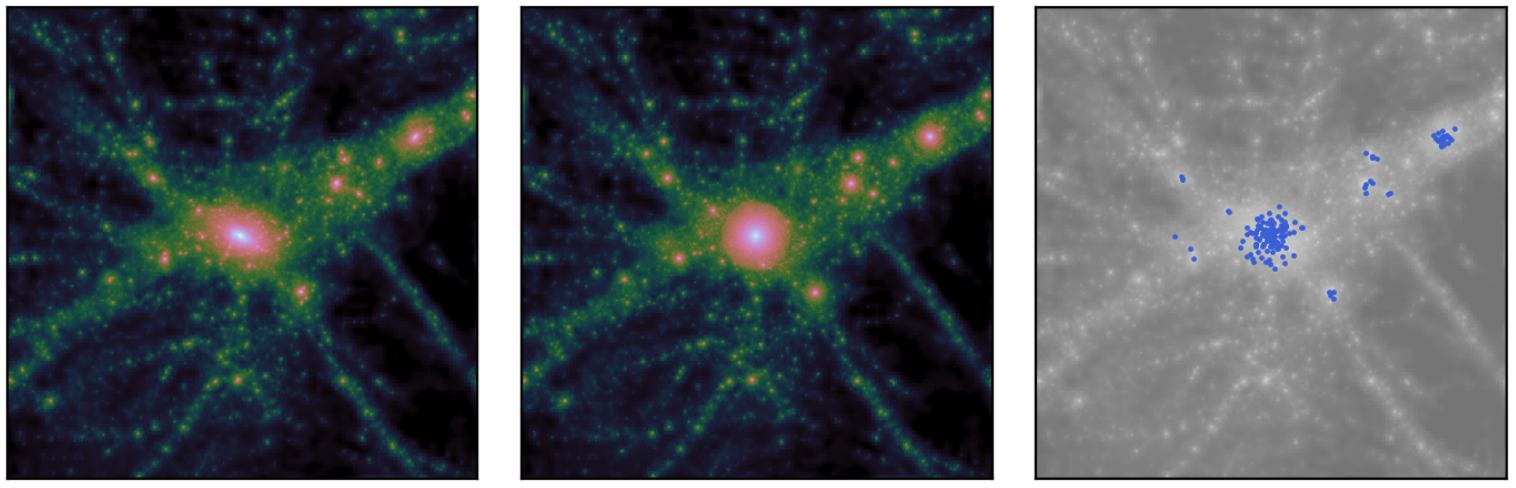
\includegraphics[scale=0.2]{img/halo.png}
    \caption{A schematic visualization of the halo model process. The left-hand panel shows the matter density field of an $N$-body simulation. The central panel shows the result of isolating all haloes identified in the simulation and replacing them with idealized spherical haloes of the same mass. The right-hand panel shows the result of populating these haloes with galaxies according to a simple galaxy-occupation prescription.}
    \label{fig:halo}
\end{figure}

We start by defining a field in the real space, $\theta_u(\bm{x})$, where $\bm{x}$ is the three-dimensional comoving position and the label $u$ stands for the field we are interested in modeling; this could be matter, halo, or galaxy over-densities. We make the assumption that everything in our field is contained within haloes distributed throughout the space with a spherically symmetric profile, $W_{u, i}$, centered at position $\bm{x}_i$, such that
\begin{equation}
    \theta_u(\bm{x}) = \sum_i N_i W_{u, i}\left(|\bm{x} - \bm{x}_i|\right)
    \label{eq:1}
\end{equation}
where the sum runs over all volume elements and $N_i = \{0, 1\}$ determines whether there is a halo center in that volume element. The Fourier transform of the field, in terms of comoving wavenumber $\bm{k}$, is given by
\begin{align}
    \label{eq:2}
    \hat{\theta}_u(\bm{k}) &= \int \theta_u(\bm{x}) e^{-i\bm{k}\cdot\bm{x}} d^3\bm{x} \\
    &= \int  \sum_i N_i W_{u, i}\left(|\bm{x} - \bm{x}_i|\right) e^{-i\bm{k}\cdot\bm{x}} d^3\bm{x} \\
    &= \sum_i N_i e^{- i\bm{k} \cdot \bm{x}_i} \int W_{u, i}(|\bm{r}|) e^{-i |\bm{k}| |\bm{r}| \cos\theta} d^3\bm{r} \\
    &= \sum_i N_i e^{- i\bm{k} \cdot \bm{x}_i} 2\pi \int_0^\infty \int_0^\pi W_{u, i}(|\bm{r}|) e^{-i |\bm{k}| |\bm{r}| \cos\theta} r^2 \sin\theta d\theta dr \\
    &= \sum_i N_i e^{- i\bm{k} \cdot \bm{x}_i} \int_0^\infty \frac{\sin(kr)}{kr} W_{u, i}(r) 4\pi r^2 dr = \sum_i N_i e^{-i \bm{k} \cdot \bm{x}_i} \hat{W}_{u, i}(k).
    \label{eq:field}
\end{align}
We assume that the properties of each halo $i$ are defined solely by its mass $M_i$, such that $W_{u, i} = W_u(M_i, r)$ and that the halo masses are distributed according to the halo-mass-distribution function $n(M)$, where $n(M) dM$ is the number of density of haloes with masses between $M$ and $M+dM$. Using this, we can find the mean value of $\theta_u(\bm{x})$ by averaging over all haloes,
\begin{align}
    \langle\theta_u(\bm{x})\rangle &= \left\langle\sum_iN_iW_u(M_i, |\bm{x} - \bm{x}_i|)\right\rangle\\
    &= \sum_i\left\langle N_iW_u(M_i, |\bm{x} - \bm{x}_i|)\right\rangle\\
    &= \sum_i \int_0^\infty dM n(M) \Delta V_i  W_u(M, |\bm{x} - \bm{x}_i) \\
    &= \int_0^\infty dM n(M) \int d^3 \bm{x}' W_u(M, |\bm{x} - \bm{x}') \\
    &= \int_0^\infty dM n(M) \int d^3 \bm{x}' W_u(M) U_u(M, |\bm{x} - \bm{x}') \\
    &= \int_0^\infty dM W_u(M) n(M),
\end{align}
where $U_u(M, x)$ is the normalized halo profile. We can define $\hat{W}_u(M, k) = W_u(M)\hat{U}_u(M, k)$. Since $U_u(M, x)$ is the normalized profile, this implies that $\hat{W}_u(M, k\to0) = \hat{W}_u(M)$. We can understand this by considering that at large scales a halo acts as a point mass, which translates to a constant in Fourier space.

We consider the correlation function between the two fields $\theta_u$ and $\theta_v$, which could be identical or different. Our fields are real, isotropic, and homogeneous such that
\begin{equation}
    \langle\theta_u(\bm{x})\theta_v(\bm{x}')\rangle = \xi_{uv}(|\bm{x} - \bm{x}'|),
\end{equation}
where $\xi_{uv}$ is the two-point correlation function and it only depends on the separation. In Fourier space, we have the power spectrum,
\begin{equation}
    \langle\hat{\theta}_u(\bm{k})\hat{\theta}^*_v(\bm{k}')\rangle = (2\pi)^3 \delta_D(\bm{k}-\bm{k}')P_{uv}(k),
\end{equation}
where $\delta_D$ is the Dirac delta function. The dimension of the power spectrum is volume times the dimensions of $\theta_u$ and $\theta_v$. If we want to remove the dependence on a volume dimension we can use,
\begin{equation}
    \Delta^2_{uv}(k) = 4\pi \left(\frac{k}{2\pi}\right)^3 P_{uv}(k).
\end{equation}
We can compute the power spectrum by inserting the fields from equation \ref{eq:field},
\begin{equation}
    \langle\hat{\theta}_u(\bm{k})\hat{\theta}^*_v(\bm{k}')\rangle = \left\langle\sum_{i,j} N_i N_j e^{-i \bm{k} \cdot \bm{x}_i} e^{i \bm{k}' \cdot \bm{x}_j} \hat{W}_{u, i}(k) \hat{W}_{v, j}(k')\right\rangle.
\end{equation}
We can separate the sums above into two parts: when $i=j$, we measure the field correlations within a single halo, the \emph{one-halo} term; when $i\neq j$, we measure field correlations between distinct haloes, called the \emph{two-halo} term.

The one-halo term is given by
\begin{equation}
    \langle\hat{\theta}_u(\bm{k})\hat{\theta}^*_v(\bm{k}')\rangle = \left\langle\sum_i N_i e^{-i (\bm{k} - \bm{k}') \cdot \bm{x}_i} \hat{W}_{u, i}(k) \hat{W}_{v, i}(k')\right\rangle,
    \label{eq:onehalo}
\end{equation}
where we used $N_i = N_i^2$. Take similar steps to what was done in finding the ensemble average of the field and the sum into continuous integrals,
\begin{align}
    \langle\hat{\theta}_u(\bm{k})\hat{\theta}^*_v(\bm{k}')\rangle &= \left\langle\sum_i N_i e^{-i (\bm{k} - \bm{k}') \cdot \bm{x}_i} \hat{W}_{u, i}(k) \hat{W}_{v, i}(k')\right\rangle \\
    &= \sum_i\left\langle\ N_i e^{-i (\bm{k} - \bm{k}') \cdot \bm{x}_i} \hat{W}_{u, i}(k) \hat{W}_{v, i}(k')\right\rangle\\
    &= \sum_i \int dM n(M) \Delta V_i e^{-i (\bm{k} - \bm{k}') \cdot \bm{x}_i} \hat{W}_{u, i}(k) \hat{W}_{v, i}(k')\\
    &= \int dM n(M) \int d^3\bm{x} e^{-i (\bm{k} - \bm{k}') \cdot \bm{x}_i} \hat{W}_{u}(k) \hat{W}_{v}(k')\\
    &= (2\pi)^3\delta_D(\bm{k} - \bm{k}') \int dM n(M) \hat{W}_{u}(k) \hat{W}_{v}(k'),
\end{align}
thus the one-halo power spectrum is,
\begin{equation}
    \label{eq:onehalop}
    P^{1h}_{uv}(k) = \int_0^\infty \hat{W}_{u, i}(M, k) \hat{W}_{v, i}(M, k) n(M) dM.
\end{equation}
The $k\to0$ limit of the one-halo term is independent of the shape of the halo profile. For this reason at large scales, the one-halo term only contributes a constant $P(k)$, so-called shot noise.

The two-halo term is defined when $i\neq j$. For this term, we have to consider the correlation between positions of haloes, $\langle N_iN_j\rangle = \xi^{ij}_{hh}(|\bm{x}_i - \bm{x}_j|)$.

\begin{align}
    \label{eq:twohalo}
    \langle\hat{\theta}_u(\bm{k})\hat{\theta}^*_v(\bm{k}')\rangle &= \left\langle\sum_i\sum_{i\neq j    } N_i N_j e^{-i \bm{k} \cdot \bm{x}_i} e^{i \bm{k}' \cdot \bm{x}_j} \hat{W}_{u, i}(M_1, k) \hat{W}_{v, j}(M_2, k')\right\rangle \\
    &= \sum_i\sum_{i\neq j}\left\langle\ N_i N_j e^{-i \bm{k} \cdot \bm{x}_i} e^{i \bm{k}' \cdot \bm{x}_j} \hat{W}_{u, i}(M_1, k) \hat{W}_{v, j}(M_2, k')\right\rangle \\
    &= \sum_i \sum_{i\neq j} \int dM_1 \int dM_2 n(M_1) n(M_2) \\
    &\nonumber \quad\quad\quad\quad\quad\quad\quad\Delta V_i \Delta V_j e^{-i \bm{k} \cdot \bm{x}_i} e^{i \bm{k}' \cdot \bm{x}_j} \hat{W}_{u, i}(M_1, k) \hat{W}_{v, j}(M_2, k')\\
    &= \int_0^\infty dM_1 \int_0^\infty dM_2~ n(M_1) n(M_2)  \hat{W}_{u}(M_1, k) \hat{W}_{v}(M_2, k') \\ \nonumber &\times \int d^3\bm{x} e^{-i \bm{k}\cdot \bm{x}} \int d^3\bm{x}' e^{i \bm{k'}\cdot \bm{x}'} \langle N(M_1, \bm{x}) N(M_2, \bm{x}')\rangle.
\end{align}
The last integral is 
\begin{equation}
    \int d^3\bm{x} e^{-i \bm{k}\cdot \bm{x}} \int d^3\bm{x}' e^{i \bm{k'}\cdot \bm{x}'} \langle N(M_1, \bm{x}) N(M_2, \bm{x}')\rangle = \langle \hat{N}(M_1, \bm{k}) \hat{N}^*(M_2, \bm{k}')\rangle = (2\pi)^3 \delta_D(\bm{k} - \bm{k}') P_{hh}(M_1, M_2, k),
\end{equation}
where $P_{hh}$ is the power spectrum of the halo centers with the shot-noise contribution subtracted. Thus, the two-halo power spectrum is
\begin{equation}
    P_{uv}^{2h}(k) = \int_0^\infty dM_1 \int_0^\infty dM_2~ n(M_1) n(M_2)  \hat{W}_{u}(M_1, k) \hat{W}_{v}(M_2, k') P_{hh}(M_1, M_2, k).
\end{equation}
As haloes are biased tracers of the underlying matter field, we can approximate the power spectrum of the halo centers as
\begin{equation}
    P_{hh}(M_1, M_2, k) = b(M_1)b(M_2)P_{mm}^{lin}(k)[1 + \beta^{nl}(M_1, M_2, k)],
\end{equation}
where $b(M)$ is the linear bias of haloes with mass $M$. The function $\beta^{nl}$ models all non-linear effects that are missing from the linear-bias-linear-field model, vanishing on large-scales: $\beta^{nl}(M_1, M_2, k\to0) = 0$. We can then write the two-halo power spectrum as
\begin{equation}
    P^{2h}_{uv}(k) = P^{lin}_{mm}(k)I^{nl}_{uv}(k) + P^{lin}_{mm}(k) \prod_{n=u, v} \left[\int_0^\infty \hat{W}_n(M, k) b(M) n(M) dM\right].
\end{equation}
It is common to set $I_{uv}^{nl}(k) = 0$ for all $k$ and therefore assume that halo bias is linear. 
\subsection{Discrete tracers}
The theory can be applied to discrete tracers, such as galaxies, with some small modifications. Modifications are necessary for two reasons: the first is that there can be a non-negligible scatter in the number of tracers that occupy haloes of the same mass; the second is that when computing the autocorrelation of a discrete tracer field, there is an automatic correlation of the field with itself at zero separation, the so-called shot noise. In configuration space, this manifests at $r=0$ in the correlation function, but in Fourier space this is spread evenly over all wavenumber, resulting in a constant shot noise power spectrum, $P^{sn} = 1/\Bar{n}$, where $\Bar{n}$ is the mean tracer number density.

Consider a field of galaxies and in particular the galaxy number density contrast, $\theta_u = \delta_g = (n_g - \Bar{n}_g)/\Bar{b}_g$. The mean number density of galaxies is defined as
\begin{equation}
    \Bar{n}_g = \langle n_g \rangle = \int_0^\infty dM n(M) N_g(M).
\end{equation}

\subsection{Selecting the Ingredients}
When using the halo model, it is necessary to make choices for the bias, halo mass function, and halo profiles. It is common to calibrate these ingredients via $N$-body simulations.

When defining haloes in simulations, it is necessary to make a boundary choice, which must be consistent when using collections of simulation-calibrated ingredients within a halo model. The fundamental choice is identifying a halo from the $N$-body simulations. The two common algorithms are friends of friends (FoF) and spherical overdensity (SO). 

The FoF scheme is simpler, with the only user-specified parameter being the `linking length', which defines the maximum distance between two particles that are considered to be part of the same halo. All particles within the linking length of at least one other particle in the halo are jointed to that halo. Typically the linking length of $b = 0.2$ times the mean-inter-particle separation is used. 

SO algorithms first choose halo centers (usually from minima in the gravitational potential, but sometimes in the density) and then grow spheres out from these peaks until a fixed overdensity threshold has been reached. With SO there are several choices to be made: the overdensity threshold (200$\Bar{\rho}$ is common) but also exactly how to define the halo centers and how to count haloes as distinct entities. SO is more common because it relates  more closely to how halo formations are thought to occur and to how haloes are identified in data sets. 

There is no single `correct' halo definition, and the best choice will depend on the observable that one is attempting to model. 

The variance in the linear matter overdensity field when smoothed on comoving scale $R$ is 
\begin{equation}
    \sigma^2(R) = \int_0^\infty 4\pi \left(\frac{k}{2\pi}\right)^3 P^{lin}(k) T^2(kR) d \ln k,
\end{equation}
where $T(kR)$ is the filter window function; the Fourier transform of the real-space top hat is
\begin{equation}
    T(x) = \frac{3}{x} (\sin x - x \cos x).
\end{equation}
The Lagrangian comoving scale, $R$, is the comoving radius of a sphere in a homogeneous Universe which contains a given mass of $M$,
\begin{equation}
    M = \frac{4}{3}\pi R^3 \Bar{\rho},
\end{equation}
thus we can relate $\sigma(R)$ in terms of mass.

The `peak height' 
\begin{equation}
    \nu(M) = \delta_c / \sigma(M),
\end{equation}
is a useful quantity that increases monotonically with the halo mass. $\delta_c(z) \simeq 1.686$ is the critical linear overdensity needed for haloes to collapse under the spherical-collapse model at redshift $z$.

The halo mass function is usually parameterized in terms of either $\sigma$ or $\nu$, rather than $M$ directly because it has been shown that the halo mass function exhibits close-to-universal behavior as a function of cosmology and redshift in terms of these variables. Analytical approaches for calculating the halo mass function rely on either peaks theory or excursion sets. 

We can write the halo mass function in terms of the peak height, by defining
\begin{equation}
    f(\nu) d\nu = \frac{M}{\Bar{\rho}} n(M) dM.
\end{equation}
If all mass is to be contained in haloes, then $f(\nu)$ integrated over all $\nu \in [0, \infty]$ should equal unity, which derives from mass conservation. A common form of $f(\nu)$ to be found in the literature is that of Sheth \& Tormen \cite{Sheth_1999}:
\begin{equation}
    f(\nu) = A[1 + (q \nu^2)^{-p}] e^{- q\nu^2/2},
\end{equation}
where $p, q$, and $A$ are fitted to simulated data. 

By far the most common form taken for the density profile is NFW
\begin{equation}
    \rho(r) = \frac{\rho_s}{r/r_s(1+r/r_s)^2},
\end{equation}
where $\rho_s$ and $r_s$ are the scale radius and density, both of which depend on the halo mass. The profile is truncated at the halo radius $r_h$ and if this truncation is not imposed then it should be noted that the total mass of the profile is infinite. The halo radius is calculated via
\begin{equation}
    M = \frac{4}{3}\pi r_h^3 \Delta_h \Bar{\rho},
\end{equation}
where $\Delta_h$ is the halo overdensity with respect to the background matter density.

The scale radius $r_s$ is usually related to $r_h$ via a concentration-mass relation: $c = r_h / r_s$.

\section{Miscellaneous}
\subsection{Cosmological Parameters}

The power spectrum has a rich structure, and its shape depends on cosmological parameters. By measuring the power spectrum, we can constrain various parameters that enter the theory calculation. The price of this multidimensional parameter space is that some of the parameters can be degenerate. Consider the following seven $\Lambda$CDM parameters:

\begin{itemize}
    \item Curvature parameter $\Omega_K = 1 - \Omega_m - \Omega_\Lambda$ often set to 0
    \item Cosmological constant $\Omega_\Lambda$
    \item Normalization of the primordial spectrum $A_s$
    \item Scalar spectral index $n_s$
    \item Reionization, parameterized by the optical depth $\tau_\text{rel}$
    \item Baryon density $\Omega_b h^2$
    \item CDM density $\Omega_c h^2$
\end{itemize}

\subsection{Tophat}

Define the real-space tophat function as
\begin{equation}
    W(\bm{x}; R) = 
    \begin{cases}
        \frac{3}{4 \pi R^3} & |\bm{x}| < R \\
        0 & \text{otherwise},
    \end{cases}
\end{equation}
then the Fourier transform of this is
\begin{align}
    \hat{W}(k;R) &= \int W(\bm{x};R) e^{-i \bm{k} \cdot \bm{x}} d^3 \bm{x} \\
    &= \frac{3}{2R^3} \int_0^R \int_0^\pi e^{-i |\bm{k}| |\bm{x}| \cos\theta} r^2 \sin\theta d\theta dr \\
    &= \frac{3}{R^3} \int_0^R \frac{\sin(kr)}{kr} r^2 dr \\
    &= \frac{3}{(kR)^3} (\sin(k R) - k R \cos(k R))
\end{align}




% Maybe I need to add one more part: Examples.
% Set style and colour later.

\newpage

% ------------------------------------------------------------------------------
% Reference and Cited Works
% ------------------------------------------------------------------------------

\bibliographystyle{IEEEtran}
\bibliography{references.bib}

% ------------------------------------------------------------------------------

\end{document}
